\documentclass{article}
\usepackage{indentfirst}
\usepackage{graphicx}
\addtolength{\oddsidemargin}{-1in} 
\addtolength{\textwidth}{2in}
\addtolength{\textheight}{1in}
\topmargin = -1in
\setlength{\parskip}{1em}

\begin{document}
\title{Stock NLP Project Report}
\author{Feiyi Ouyang}
\date{}
\maketitle
\section{Introduction}
In the information era, the more information you have the more likely you're gonna win. It can not fit stock market more. One of the most urgent need of stock traders is to retrieve information about the whole picture of the market and how each stock performs. However, time is limited and news come out every minute. It's impossible to check out ginormous source of information manually. Facing such a chaos world, how to collect and extract useful information about stock market has always been a temptating but challenging task. 

On the other hand, latest advances in information collecting and analyzing field, like NLP, machine learning offers great opportunities for solving these challenges. Late last year, a group of MicroSoft researchers has successfully predicted stock market by analyzing publicly available documents like 10-K reports using natural language processing and machine learning techniques [1]. The success of the project provided thrilling prospect that digging public resources provides the key to the secret of the stock market with the help of modern analyzing technologies. 

This project built a stock analyzing and summarizing tool by integrating web crawling, NLP parsing, and information retrieval model ranking techniques. The project provides answers to the following questions: 

\begin{itemize}
  \item What are the most popular topics of a certain day?
  \item What is the market\'s response to a stock (positive / negative)?
  \item What are the most related articles of a stock or a query?
\end{itemize}

\section{Overview design}
We chose an authoritative Chinese finance website CNFOL.com which provides news of public companies as the information source. We chose the website because it provides a good capture of activities of public companies, as well as people's response to it.

The project is divided into the crawling and querying process. For the crawling process, the crawler go through the following stages:

\begin{itemize}
  \item Crawl the articles of all the posts in a given time period. The crawling process is scheduled as a daemon job run at specific time everyday. 
  \item Parse the articles and index the terms. The indexed result is stored into a database.
\end{itemize}

The querying process goes through the following stages:

\begin{itemize}
  \item Client sends queries to server.
  \item Server parses the queries, calculates related statistics, and retrieves documents in response to queries
  \item Server sends result in json format to the client
  \item Client displays the data in a user friendly way
\end{itemize}

\section{Investigation over available solutions}
\subsection{Crawling}
There are many open source web crawler libraries, like Scrapy in python and Crawler4j in Java. However, considering that the data we need to crawl is not big if we just run the crawler everyday, we decide to implement the crawler ourselves.

For our crawler, we need a html client which opens a connection and a HTML parser to select specific DOM elements. Jsoup provides good interface for these use cases [2].

\subsection{Parsing}
Unlike English where each word is a individual unit, Chinese words can be formed by undefined number of characters. Further more, Chinese words are not separated by splitters. These two characteristics make it hard to parse chinese words.

HanLP [3], a NLP library for Chinese language is an ideal tool for our parsing. Not only does it provide robust segmenter, POS tagger, but also customized dictionary, which allows users to mark words with specified taggers. This flexibility enables us to distinguish our own word groups like stock names, words that describe positive or negative stock trend, etc.

\subsection{Indexing, storing, and querying}
The most popular indexing tool for search engines is ElasticSearch, which nicely bundles indexing, ranking, and querying functionalities and provides an easy user interface. It can be seen as a database, but is more powerful in supporting various forms of queries and full text search, which are not supported by database like MongoDB. 

However, ElasticSearch is challenging for Chinese documents. Although Smart Chinese Analysis plugin helps segmenting Chinese, it doesn't not offer POS tagging and customized dictionary as HanLP do. Furthermore, some people criticize that ElasticSearch is not ready to be the main storage of data [4]. Although it outperforms databases in indexing and reading, it is not optimized for maintenance like re-importing and changing data structure.

On the other hand, the principle behind ElasticSearch is quite simple[5]. The statistics needed to compute scores for each query-document pair is easy to calculate if data is stored carefully. Here, MongoDB provides a elegant solution for flexible data storage using Json without specifying schema. Furthermore, there's free MongoDB instance hosting on AWS (mLab) which largely reduces the need to maintain. Thus, rather than using ElasticSearch, we build the indexer ourselves, store them to MongoDB, and calculate scores by implementing information retrieval ranking functions. Although it increases the complexity of implementation, it is a good opportunity to learn the underlying theories and helps making the project lighter (less dependencies).

\subsection{User interface and communication with search engine server}
A search engine without a good user interface is disappointing. Instead of a command line interface, we provide a graphic interface to send user queries and display received data in a good format. Web pages are ideal for this purpose, and React simplifies the process of make a light, quick web application. 

Web pages can only communicate with external resources over HTTP. Thus, we need another server to expose HTTP endpoint to respond to request and run the search engine. Given that most of our search engine is written in Java, we finally choose to build a Java socket to expose the HTTP end points to client.

\subsection{Why we chose Java}
There are good libraries in Python and JavaScript for each stage of the project, but Java is the one that can do all the job. For example, Python is good for the crawling stage because of the Scrapy framework, but it is not powerful when it comes to the complex parsing and indexing stage. JavaScript is good for implementing servers on NodeJS platform, but it does not have good support for HanLP library. In addition to library supports, a compiled language like Java is more efficient than a scripting language like Python and JavaScript for the indexing phase, which is computationally intensive.

\section{Implementation (refer to supplementary material for the pipeline)}
\subsection{Customized dictionaries}
We creat three customized dictionaries for HanLP parser to tag segmented Chinese words. The stock name dictionary contains all the stock names with our own tag "sn". The positive / negative words dictionary contains all the sentimental words used to describe stock market, and these words are tagged as "pos" and "neg", respectively. The stop words are collected from several common stop word lists online and tagged "sw".

\subsection{Java classes [source code: 6]}
\subsubsection{Crawler and MetaData}
The Crawler class establishes a connection with the seed page, crawls a list of article posts, and constructs a queue of MetaData, which summarizes the title, url, and time stamp of each post. As the seed page uses dynamic rendering, which pulls more data when users drag to the buttom, we can not extract links only based on static html. Instead, we monitor the network activity in Chrome debug tools when the page renders new contents and find the http endpoint to retrieve JSON format of article posts. We launch http requests to that endpoint specifying which page of data we want and get history data (eg, posts two days ago).

For each MetaData we called `parse` method on themselves. The parsing pipeline involves the following processes:
\begin{enumerate}
  \item Crawl the article text from the url.
  \item Pass the article text through NLP segmenter and get a list of words with POS taggers.
  \item Filter words with stop words tags and punctuation.
  \item Extract contexts for each the filtered term lists. Each context is centered about stock names and has a length of at least 20 words. If multiple contexts overlap, we merge them into one.
  \item Index terms and docs with their hashes. Create term entrys, document entrys, and post entrys. The three kinds of entrys has the following JSON format:
  \begin{itemize}
    \item term: \par
      \texttt{\detokenize{"_id":<term_hash>,"term":<term_word>}} \par
    \item document:\par
      \texttt{\detokenize{"_id":<doc_url_hash>,"url":<doc_url_string>,}} \par
      \texttt{\detokenize{"title":<doc_title>,"tiem":<time_stamp>,}} \par
      \texttt{\detokenize{"pos":<number_of_positive_words>,"neg":<number_of_negative_words>,}} \par
      \texttt{\detokenize{"snippet":<snippets_list>,"relatedStocks":<stock_name_string>}}\par
    \item post:\par
      \texttt{\detokenize{"term":<term_hash>,"doc":<doc_hash>,}}\par
      \texttt{\detokenize{freq":<term_frequency_in_doc>,"norm":<position_of_term>}}
  \end{itemize}
  \item Write the above collections to an AWS instance of MongoDB hosted on the cloud in batch mode. 
\end{enumerate}

\subsubsection{Query}
The Query class implements a static method `calDf' to calculate document frequency for each term in each collection, by counting the number of postings containing term hash. These document frequencies (for each term) are stored into seperate collections. We store this helper data to enhance real time retrieval, which simulates the caching mechanism. This function is scheduled to run as a daemon process everyday.

The Query class resolves three kinds of queries at real time: 
\begin{itemize}
  \item Query popular words: find the top 10 terms in the document frequency collection of each day. 
  \item Query stock: find all the documents with the `relatedStocks' field containing the stock. Calculate the total number of positive and negative words as an index of market response. Also return all the related stocks.
  \item Common query: replicate step 2 and 3 in parsing pipeline to get list of terms. For each term, calculate a score for all the documents containing this term. The score is calculated as:\\
  \textbf{score(q,d) = coord(q,d) * sum of (tf(t in d) * idf(t) * idf(t) * boost * norm(t,d)) (for t in q)} \\
  where:
  \begin{itemize}
    \item `term(t,d)' is retrieved from the `frequency' field of the match posting; 
    \item `idf(t)' is calculated using df(t) which is retrieved from the matched document frequency entry; 
    \item `coord(q,d)' is the sum of tf(t,d) of all query terms; 
    \item `boost' is a measure of freshness (eg, 4 = document of today; 3 = document of yesterday, etc)
    \item `norm(t,d)' is a measure of term position weight (eg, 3 = if term in context; 2 = if term in title; 1 = otherwise)
  \end{itemize}
  Return the documents with the top scores.
\end{itemize}

\subsubsection{Server}
The server class opens a socket on port 9090 and keeps reading the socket input stream. It parses the arguments of input stream, calls corresponding Query functions, and returns the query results in JSON format

\subsection{React client}
The React client provides three search boxes, asking parameters for three queries respectively. Getting responses from the Java server, the React client parses the data and display data beautifully. 

\section{Result, Evaluation and Improvements}
\begin{itemize}
  \item Popular words query: We found that the top words retrieved contain too much noise. Although we filtered out common words in the stop words process, we did not filter the common words used in the financial world, like companies, stock holders. To actually extract the hot topic words, we need to combine other indexes rather than using pure document frequency. For example, we can compare popular words between days and only select those which have high document frequecies recently.
  \item Stock query: First, we analyzed if the total number of sensational words (positive / negative words) captures the stock market. We found that there were many trend predicting words we didn't capture. Thus, we need to manually check the parsed articles and add more sensational words to our dictionary. Second, we evaluated if the snippets captured the essence of the article. By looking at the snippets along, it's easy to get the main idea of the article. However, the current snippets are still too long and contain too much noise. We should consider developing another filter over the extracted contexts to remove those information that are not useful. Further more, we should consider build snippets with the unfiltered terms in stead of filtered terms to make it easier to understand for users. 
  \item Common query: We found that the returned documents contained a high percentage of query words, which is consistent with our hypothesis. Also, we found that the documents with high term frequencies for all the words in the query had higher scores than those with extremely high frequency for one of the query words, which is also consistent with our assumption. However, we should normalize documents by it's length to prevent bias towards longer documents.
\end{itemize}


\section{Supplementary Material}
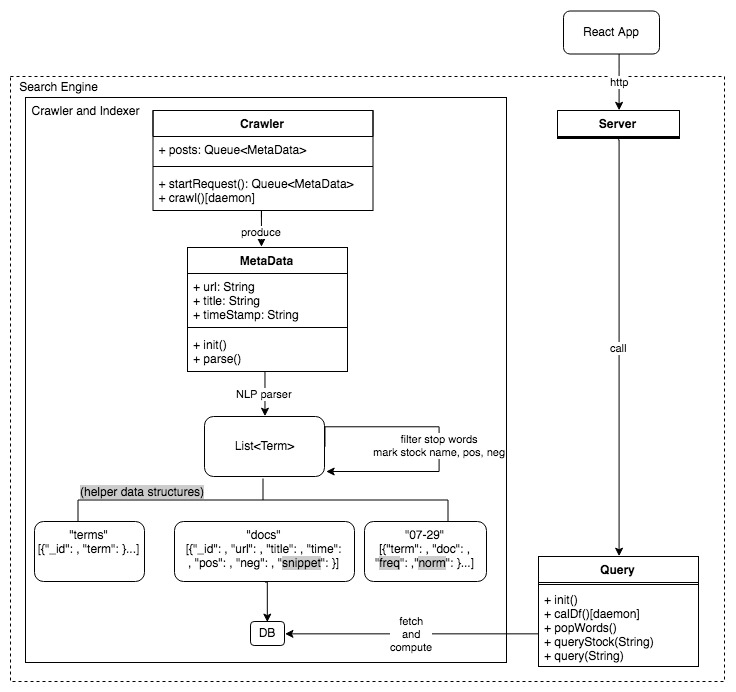
\includegraphics[width=7in]{StockNLP_Pipeline}

\section{References}
\vspace{-5pt}\hspace{-15pt}[1] MicroSoft stock prediction project: https://www.microsoft.com/developerblog/2017/12/04/predicting-stock-performance-deep-learning\par
\vspace{-5pt}\hspace{-15pt}[2] Jsoup: https://jsoup.org\par
\vspace{-5pt}\hspace{-15pt}[3] HanLP: https://github.com/hankcs/HanLP\par
\vspace{-5pt}\hspace{-15pt}[4] ElasticSearch compared to MongoDB: https://www.ip-label.co.uk/performance-wire/mongodb-and-elasticsearch\par
\vspace{-5pt}\hspace{-15pt}[5] ElasticSearch scoring principle: https://www.ip-label.co.uk/performance-wire/mongodb-and-elasticsearch\par
\vspace{-5pt}\hspace{-15pt}[6] The source code is stored here: https://github.com/fayeoyaee/SearchEngine/tree/master/stockNLP\par
\end{document}
